\documentclass{standalone}
\usepackage{Note}
\begin{document}
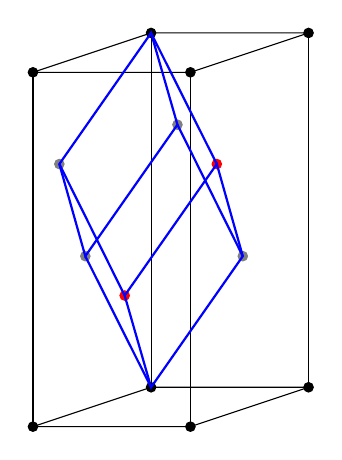
\begin{tikzpicture}[scale=0.5]
\coordinate (O)  at (0,0);
\coordinate (A)  at (4,0);
\coordinate (B)  at (7,1);
\coordinate (C)  at (3,1);
\coordinate (O1) at (0,9);
\coordinate (A1) at (4,9);
\coordinate (B1) at (7,10);
\coordinate (C1) at (3,10);
\draw (O)--(A)--(B)--(C)--cycle;
\draw (O1)--(A1)--(B1)--(C1)--cycle;
\draw (O)--(O1);
\draw (A)--(A1);
\draw (B)--(B1);
\draw (C)--(C1);

\coordinate (R1) at (4.67,6.67);
\coordinate (R2) at (2.33,3.33);
\coordinate (R3) at (5.33,4.33);
\coordinate (R4) at (1.33,4.33);
\coordinate (R5) at (0.67,6.67);
\coordinate (R6) at (3.67,7.67);


\foreach \p in {O,A,B,C,O1,A1,B1,C1}
{
    \filldraw (\p) circle (0.12);
}
\foreach \p in {R3,R4,R5,R6}
{
    \filldraw[gray] (\p) circle (0.12);
}
\foreach \p in {R1,R2}
{
    \filldraw[red] (\p) circle (0.12);
}
\draw[blue,thick] (C) -- (R2) -- (R1) -- (R3) --cycle;
\draw[blue,thick] (C1) -- (R6) -- (R4) -- (R5) --cycle;
\draw[blue,thick] (C) -- (R4);
\draw[blue,thick] (R1) -- (C1);
\draw[blue,thick] (R2) -- (R5);
\draw[blue,thick] (R3) -- (R6);
\end{tikzpicture}
\end{document}